\documentclass[a4paper,10pt]{article}
\usepackage{geometry}
\usepackage{tcolorbox}
\usepackage{listings}
\usepackage[table]{xcolor}
\usepackage{amsmath}
\usepackage{graphicx}
\usepackage{wrapfig}
\usepackage{hyperref}
\usepackage{enumitem}
\usepackage{multicol}
\usepackage{tikz}
\usepackage{array}
% \usepackage{paralist}

\geometry{
    top=1.2cm,
    bottom=1.5cm,
    left=1.3cm,
    right=1.3cm
}

\definecolor{codegray}{rgb}{0.9,0.9,0.9}
\definecolor{darkblue}{rgb}{0,0,0.5}

\setlength{\tabcolsep}{2pt}

\lstdefinestyle{mystyle}{
    backgroundcolor=\color{codegray},   
    commentstyle=\color{darkblue},
    keywordstyle=\color{blue},
    numberstyle=\tiny\color{gray},
    stringstyle=\color{red},
    basicstyle=\ttfamily\footnotesize,
    breaklines=true,
    numbers=left,                    
    numbersep=5pt,                  
    showspaces=false,                
    showstringspaces=false,
    showtabs=false,                  
    tabsize=4
}
\lstset{style=mystyle}
\newtcolorbox{definitionbox}[1]{colback=blue!5!white,colframe=blue!75!black,title=#1}
\hypersetup{
    colorlinks=true,
    linkcolor=blue,
    filecolor=magenta,      
    urlcolor=blue,
}
\setlist[itemize]{nosep}

\newcommand{\hl}[1]{\textcolor{violet}{\textit{#1}}}
\renewcommand{\arraystretch}{0.8}
\newcommand{\tabletitle}[1]{\multicolumn{2}{c}{\textbf{#1}}}

\title{\huge Curs Arhitectura Sistemelor de Calcul - FMI}
\author{
  Matei-Iulian Cocu\\
  \texttt{matei-iulian.cocu@s.unibuc.ro}
  \and
  Ștefan Chiper\\
  \texttt{stefan.chiper@s.unibuc.ro}
} \date{}
\renewcommand*\contentsname{\large\bfseries Cuprins}

\begin{document}
\maketitle
\setcounter{tocdepth}{2}
\tableofcontents
\thispagestyle{empty}
\newpage

\section{Prolog}
\begin{wrapfigure}{r}{0.3\textwidth}
    \centering
    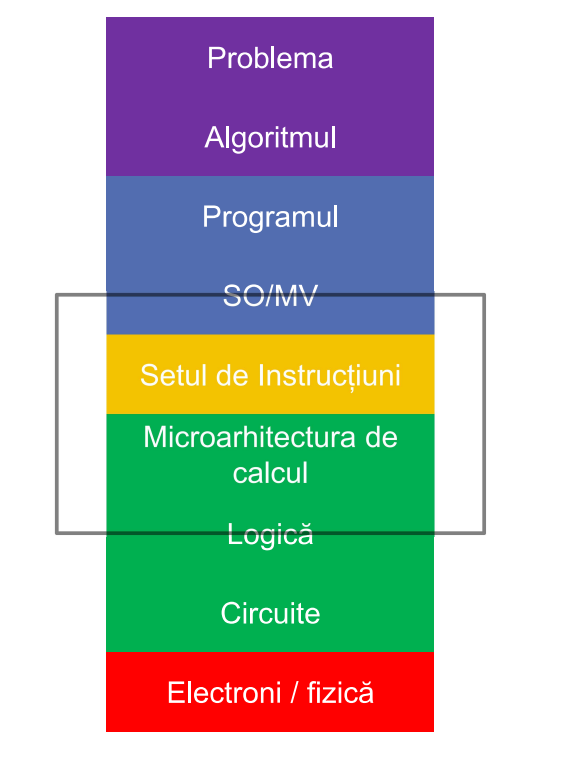
\includegraphics[width=0.25\textwidth]{resources/ierarhia.png}
    \caption{Ierarhia Abstractizării}
\end{wrapfigure}

\quad Acest document este o compilație succintă a cursului de \textbf{Arhitectura Sistemelor de Calcul}, o materie de bază a primului an în cadrul specializării Informatică din cadrul Facultății de Matematică și Informatică București.
\quad Documentul conține toată materia imperativă cursului, cât și alte adăugiri relevante materiei de studiu. \newline \quad Fiind un curs introductiv, acesta introduce noțiuni importante în următoarele domenii:
\begin{itemize}
    \item securitate informatică
    \begin{itemize}
        \item Reverse Engineering (RE)
        \item hacking
    \end{itemize}
    \item optimizare
    \begin{itemize}
        \item dezvoltare a jocurilor
        \item Machine Learning (ML/AI)
    \end{itemize}
    \item debugging
    \item dezvoltare software \textit{low-level}
    \begin{itemize}
        \item dezvoltare pentru sisteme embedded
        \item dezvoltare pentru sisteme de operare
    \end{itemize}
\end{itemize}
\textbf{Referințe bibliografice generale}
\begin{itemize}
    \item \href{https://www.google.com/url?sa=t&rct=j&q=&esrc=s&source=web&cd=&cad=rja&uact=8&ved=2ahUKEwjt2ZXGo4CPAxW2SfEDHZXIFQ8QFnoECC8QAQ&url=https%3A%2F%2Fia601209.us.archive.org%2F24%2Fitems%2FComputerOrganizationAndDesign3rdEdition%2F-computer%2520organization%2520and%2520design%25203rd%2520edition.pdf&usg=AOvVaw1pgFBveFHAibz19Tz7R-6D&opi=89978449}{D. Patternson and J. Hennessy, Computer Organisation and Design}
    \item \href{https://www.google.com/url?sa=t&rct=j&q=&esrc=s&source=web&cd=&ved=2ahUKEwjv3JPjpICPAxWNQ_EDHc0gLvoQFnoECB0QAQ&url=https%3A%2F%2Farchive.org%2Fdownload%2FProfessional_Assembly_Language_2005%2FProfessional_Assembly_Language_2005.pdf&usg=AOvVaw3TJSBH1Y0pcpnMmrMsjSPH&opi=89978449}{R. Blum, Professional Assembly Language}
\end{itemize}

\section{Evoluția sistemelor de calcul. Sistemul binar}
\subsection{Scurt istoric al sistemelor de calcul}
\begin{multicols}{2}
\subsubsection{Blaise Pascal (1623 - 1662)}
În 1642, crează \textbf{Pascaline}: un calculator mecanic capabil de adunări și scăderi (utilizat pentru calcul de taxe). Nefiind o mașină practică, mai puțin de 50 de astfel de mașini au fost create, fiind utilizată mai degrabă pe post de "jucărie" a aristocraților. Bineînțeles, acesta a fost un important contribuitor al secolului XVII, limbajul \textbf{Pascal} fiind numit în onoarea acestuia. 
\subsubsection{Gottfried Wilhelm Von Leibniz (1646 - 1716)}
Având contribuții numeroase în domenii precum , două dintre contribuțiile sale majore în acest domeniu fiind:
\begin{itemize}
    \item studiul sistemului binar;
    \item extinderea mașinii Pascaline, adăugând operațiile de înmulțime și împărțire - tot o mașină mecanică, creată în 1673.
\end{itemize}
\subsubsection{George Boole (1815 - 1864)}
\begin{itemize}
    \item scrie \textit{"The Laws of Thought"} (1854)
    \item introduce \textit{logica booleană} și analizează operațiile de bază \textit{(negația (NOT), conjuncția (AND), disjuncția (OR), disjuncția exclusivă (XOR))}
\end{itemize}
\subsubsection{Charles Babbage (1791 - 1871)}
\begin{itemize}
    \item proiectează teoretic Mașina Diferențială \textit{(Difference Engine No. 2)}
    \item design-ul este realizat de abia în 1991
    \item reprezintă prima mașină de calcul \textit{(mecanică)} programabilă
    \item asemenea prototipuri ajungea la greutatea de gradul tonelor, această mașină ajungând să cântărească peste 13 tone
\end{itemize}
\subsubsection{Ada Lovelace (1815 - 1852)}
\begin{itemize}
    \item colaboratoare a lui \textit{Babbage}
    \item scrie primul program, calculează \textit{numere Bernoulli}
    \item nu existau limbaje de programare, programul reprezentând \textit{o serie de pași de executat de o mașină}
    \item este considerată primul "programator"
\end{itemize}
\subsubsection{Konrad Zuse (1910 - 1995)}
\begin{itemize}
    \item introduce o serie de calculatoare: Z1, Z2, Z3 și Z4
    \item primele prototipuri în 1940-1941, folosesc \textit{sistemul binar}, instrucțiunile acestora fiind stocate pe o \textit{bandă perforată}
    \item introduce reprezentarea și calculul în \textit{virgulă mobilă}
    \item majoritatea efortului acestuia a fost făcut în izolare (1936-1945), dat fiind contextul cel de-al Doilea Război Mondial
\end{itemize}
\subsubsection{Alan Turing (1912 - 1954)}
\begin{itemize}
    \item celebru pentru publicul larg pentru contribuția lui în spargerea rapidă a mesajelor \href{https://en.wikipedia.org/wiki/Cryptanalysis_of_the_Enigma}{Enigma} utilizând mașina "The Bombe" (calcul brut cu scopul de a reduce numărul de posibilități în decriptarea mesajelor)
    \item introduce Mașina Turing
    \begin{itemize}
        \item un model teoretic pentru a implementa orice algoritm
        \item conceptul de Turing-complete (un sistem care poate recunoaște și analiza seturi de reguli pentru manipularea datelor - o cantitate infinită, teoretic)
    \end{itemize}
\end{itemize}
\end{multicols}
\subsubsection{John von Neumann (1903 - 1957)}
\begin{wrapfigure}{r}{0.3\textwidth}
    \centering
    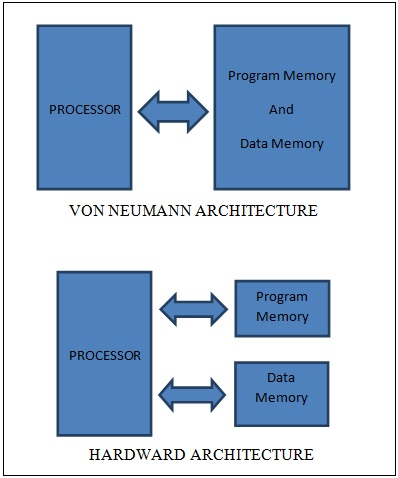
\includegraphics[width=0.25\textwidth]{resources/von_neumann_and_harvard_architecture.jpg}
    \caption{Ierarhia Abstractizării}
\end{wrapfigure}
Considerat unul dintre cei mai influenți matematicieni ai ultimului secol, John von Neumann a adus contribuții fundamentale în numeroase domenii. În domeniul calculatoarelor, cele mai importante sunt:
\begin{itemize}
    \item \textbf{contribuția la crearea primului calculator electronic ENIAC (Electronic Numerical Integrator And Computer), 1939-1944}
    \item \textbf{îmbunătățirea ENIAC, ajutând la crearea EDVAC (Electronic Discrete Variable Automatic Computer), sistemul este binar și are programe stocate}
    \item \textbf{introducerea arhitecturii von Neumann} - diferența dintre aceasta și \textit{arhitectura Harvard} fiind utilitatea în sine:
    \begin{itemize}
        \item arhitectura Harvard prioritizează viteza de procesare, având la dispoziție două seturi de memorie separate;
        \item arhitectura von Neumann conferă sistemului de calcul o flexibilitate superioară arhitecturii latente;
        \item uzual, arhitectura von Neumann este folosită în sistemele de calcul \textit{general purpose} (desktop-uri, laptop-uri), pe când arhitectura Harvard este folosită de obicei în scopuri specifice (ex.: mașini de spălat, sisteme anti-furt, tehnologie militară)
    \end{itemize}
\end{itemize}
\begin{multicols}{2}
\subsubsection{Claude Shannon (1916 - 2001)}
\begin{itemize}
    \item \textbf{considerat "părintele teoriei informației"}
    \item \textbf{contribuții excepționale atribuite}
    \begin{itemize}
        \item demonstrează faptul că problemele de logică Booleană pot fi rezolvate cu circuite electronice
        \item teorema de eșantionare \href{https://en.wikipedia.org/wiki/Nyquist–Shannon_sampling_theorem}{Shannon-Nyquist} (de la analog la digital și înapoi, fără pierderi de informație)
        \item inventează teoria informației
    \end{itemize}
\end{itemize}
\subsubsection{Post-Shannon}
\begin{itemize}
    \item după cel de-al Doilea Război Mondial, cercetarea în domeniul calculatoarelor începe în ritm exponențial
    \item actorii importanți în domeniu au devenit grupurile profesionale (ex.: IEEE, ACM, Bell Labs) și statele (ex.: Statele Unite, Germania, Marea Britanie, programele de cercetare DARPA)
\end{itemize}
\subsubsection{Alte personalități (și concepte) importante}
\begin{itemize}
    \item \textbf{Al-Khwarizmi (780 - 845):} astronom/astrolog persan, matematician, inventatorul termenului "algoritm";
    \item \textbf{Grace Hopper (1906 - 1992):} creatorul primului compilator, dezvoltator al limbajului COBOL;
    \item \textbf{Margaret Hamilton (1936 - ):} software engineer, a condus echipa care a dezvoltat software-ul de zbor pentru misiunile Apollo;
    \item \textbf{Barbara Liskov (1939 - ):} distributed computing, limbajul CLU, principiul substituției Liskov, premiul Turing 2008, prima femeie doctorandă în CS/IT;
    \item \textbf{Howard H. Aiken (1900 - 1973):} ASCC, Mark I, Mark II, Mark III, Mark IV;
    \item \textbf{Richard Hamming (1915 - 1998):} coduri de corecție a erorilor, distanța Hamming, premiul Turing 1968;
    \item \textbf{RSA (1977):} Ron Rivest, Adi Shamir, Leonard Adleman - \textbf{criptografie} cu cheie publică;
    \item \textbf{Diffie-Hellman (1976):} Whitfield Diffie, Martin Hellman, Ralph Merkle - metodă matematică de generare securizată a unei chei criptografice simetrice;
    \item \textbf{UNIX - Ken Thompson, Dennis Ritchie:} sistem de operare inițiat de un grup de programatori de la Bell Labs în 1969, scris în limbajul C, influențând numeroase sisteme de operare ulterioare (inclusiv Linux și MacOS);
    \item \textbf{Linus Torvalds:} creatorul nucleului Linux în 1991, inițial ca un proiect personal, devenind ulterior unul dintre cele mai importante sisteme de operare open-source;
    \item \textbf{Richard Stallman:} fondatorul mișcării software liber, inițiatorul proiectului GNU în 1983, care a contribuit semnificativ la dezvoltarea software-ului open-source;
    \item \textbf{Brian Kernighan și Dennis Ritchie:} co-creatori ai limbajului de programare C;
    \item \textbf{Larry Page (CEO) și Sergey Brin (CTO):} Google, Alphabet Incorporated.
\end{itemize}
\end{multicols}

\subsection{Sistemul binar - baza sistemelor moderne de calcul}
\begin{multicols}{2}
\begin{itemize}
    \item bit = \hl{bi}nary digi\hl{t}
    \item sistem de numărare cu \hl{baza B = 2}
    \item avem disponibile două cifre: \hl{0} și \hl{1}
\end{itemize}
\vspace{0.1cm}
$x = \sum_{i=0}^{N-1} b_i 2^i$, unde \hl{N} este numărul de biți folosiți în reprezentare
\vspace{0.5cm}
\begin{tabular}{|>{\color{green}}l*{10}{|c}|}
\hline
bit $b_i$: & \cellcolor{blue!50}\color{white}0 
            & \cellcolor{blue!50}\color{white}1 
            & \cellcolor{blue!50}\color{white}1 
            & \cellcolor{blue!50}\color{white}1 
            & \cellcolor{blue!50}\color{white}1 
            & \cellcolor{blue!50}\color{white}0 
            & \cellcolor{blue!50}\color{white}0 
            & \cellcolor{blue!50}\color{white}0 
            & \cellcolor{blue!50}\color{white}1 \\ \hline
        {\color{green}2$^i$:} 
            & $2^8$ & $2^7$ & $2^6$ & $2^5$ & $2^4$ & $2^3$ & $2^2$ & $2^1$ & $2^0$ \\
\hline
\end{tabular}

\noindent În exemplul de mai sus: $0 \times 2^8 + 1 \times 2^7 + 1 \times 2^6 + 1 \times 2^5 + 1 \times 2^4 + 0 \times 2^3 + 0 \times 2^2 + 0 \times 2^1 + 1 \times 2^0 = 241$ \hspace{1cm} (avem \textit{N = 9}, dar în realitate se poate reduce la \textit{N = 8})
\vspace{0.15cm}

\noindent Intuiția noastră este în baza \textit{B = 10}, dar este folositor să abstractizăm și să considerăm baza generală \textit{B}; așadar, în baza \textit{B} avem:
\begin{itemize}
    \item cifre de la \textit{0} la \textit{B-1} (restul se numesc numere)
    \item reprezentarea este $x = \sum_{i=0}^{N-1} b_i B^i$
    \item bitul $b_0$ se numește \hl{Least Significant Bit (LSB)} iar bitul $b_{N-1}$ se numește \hl{Most Significant Bit (MSB)}
    \item reprezentarea unui număr din baza 10 în baza B se face prin \textit{împărțiri succesive cu B și păstrare de rest}
\end{itemize}
\noindent \hl{\textbf{Regula generală:} când trecem din baza B în baza $B^p$ trebuie doar să grupăm noul număr în câte p cifre}
\vspace{0.15cm}

\textbf{Numere întregi negative}
\begin{tabular}{|>{\color{green}}l*{10}{|c}|}
\hline
bit $b_i$: & \cellcolor{blue!50}\color{white}1 
            & \cellcolor{blue!50}\color{white}1 
            & \cellcolor{blue!50}\color{white}1 
            & \cellcolor{blue!50}\color{white}1 
            & \cellcolor{blue!50}\color{white}0 
            & \cellcolor{blue!50}\color{white}0 
            & \cellcolor{blue!50}\color{white}0  
            & \cellcolor{blue!50}\color{white}1 \\ \hline
        {\color{green}2$^i$:} 
            & $-2^7$ & $2^6$ & $2^5$ & $2^4$ & $2^3$ & $2^2$ & $2^1$ & $2^0$ \\
\hline
\end{tabular}

$x = - b_{n-1} 2^{n-1} + \sum_{i=0}^{n-2}b_i 2^i$

\noindent În exemplul de mai sus: $-1 \times 2^7 + 1 \times 2^6 + 1 \times 2^5 + 1 \times 2^4 + 0 \times 2^3 + 0 \times 2^2 + 0 \times 2^1 + 1 \times 2^0 = -15$
\end{multicols}

\begin{wrapfigure}
{r}{0.3\textwidth}
    \centering
    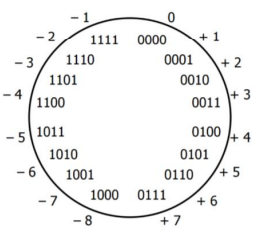
\includegraphics[width=0.25\textwidth]{resources/cerc_num_intregi.png}
\end{wrapfigure}
\noindent \textbf{Reprezentarea în complement față de 2:}
\begin{itemize}
    \item numere în intervalul $[-2^{N-1}, 2^{N-1}-1]$
    \item se pierde un bit pentru semn, dar este optim: \textbf{MSB} este semnul, \textbf{restul biților} reprezintă valoarea
    \item pentru a obține reprezentarea în complement față de 2 a unui număr negativ, se inversează toți biții și se adaugă 1
    \item motivul pentru care folosim acest sistem în complement față de 2 este că \hl{algoritmul de adunare} este la fel ca pentru numere naturale
\end{itemize}
\vspace{0.2cm}

\noindent \textbf{Adunări/Scăderi} pe numere naturale și întregi:
\begin{itemize}
    \item se adună bit cu bit, de la LSB la MSB; se păstrează un \textbf{carry} dacă suma depășește baza (2)
    \item \textbf{Overflow} apare când rezultatul nu poate fi reprezentat cu numărul de biți alocați
    \item \textbf{Underflow} apare când rezultatul este mai mic decât cel mai mic număr reprezentabil
\end{itemize}
\hrule
\vspace{0.2cm}
\noindent \textbf{Extinderea} numărului de biți:
\begin{itemize}
    \item \textbf{Zero-Extension} - pentru numere naturale, se adaugă biți 0 în partea stângă (e.g., 6 biți $\rightarrow$ 8 biți: 001101 $\rightarrow$ 00001101)
    \item \textbf{Sign-Extension} - pentru numere întregi, se adaugă biți egali cu MSB în partea stângă (e.g., 6 biți $\rightarrow$ 8 biți: 111101 $\rightarrow$ 11111101)
\end{itemize}

Logica binară (unde 0 = False, 1 = True) implică operații de bază esențiale în arhitectura sistemelor de calcul pentru funcționarea circuitelor digitale și a procesorului: NOT \hl{(negație)}, AND \hl{(conjuncție)}, OR \hl{(disjuncție)} și XOR \hl{(disjuncție exclusivă)}.
\vspace{0.3cm}

\begin{center}
\begin{minipage}[t]{0.24\textwidth}
    \centering
    \begin{tabular}{|c|c|}
        \hline
        \multicolumn{2}{|c|}{\textbf{NOT}} \\
        \hline
        \textbf{A} & \textbf{$\neg$ A} \\
        \hline
        0 & 1 \\
        1 & 0 \\
        \hline
    \end{tabular}
\end{minipage}\hfill
\begin{minipage}[t]{0.24\textwidth}
    \centering
    \begin{tabular}{|c c|c|}
        \hline
        \multicolumn{3}{|c|}{\textbf{AND}} \\
        \hline
        \textbf{A} & \textbf{B} & \textbf{A $\land$ B} \\
        \hline
        0 & 0 & 0 \\
        0 & 1 & 0 \\
        1 & 0 & 0 \\
        1 & 1 & 1 \\
        \hline
    \end{tabular}
\end{minipage}\hfill
\begin{minipage}[t]{0.24\textwidth}
    \centering
    \begin{tabular}{|c c|c|}
        \hline
        \multicolumn{3}{|c|}{\textbf{OR}} \\
        \hline
        \textbf{A} & \textbf{B} & \textbf{A $\lor$ B} \\
        \hline
        0 & 0 & 0 \\
        0 & 1 & 1 \\
        1 & 0 & 1 \\
        1 & 1 & 1 \\
        \hline
    \end{tabular}
\end{minipage}\hfill
\begin{minipage}[t]{0.24\textwidth}
    \centering
    \begin{tabular}{|c c|c|}
        \hline
        \multicolumn{3}{|c|}{\textbf{XOR}} \\
        \hline
        \textbf{A} & \textbf{B} & \textbf{A $\oplus$ B} \\
        \hline
        0 & 0 & 0 \\
        0 & 1 & 1 \\
        1 & 0 & 1 \\
        1 & 1 & 0 \\
        \hline
    \end{tabular}
\end{minipage}
\end{center}


\subsection{Lectură suplimentară}
\begin{itemize}
    \item \textbf{PH Book}:
        \begin{itemize}
            \item \textbf{2.4:} Signed and Unsigned Numbers
            \item \textbf{2.17:} Real Stuff: x86 Instructions
            \item \textbf{3.2:} Addition and Subtraction
        \end{itemize}
    \item \href{https://tfinley.net/csarch-notes/}{Thomas Finley Course Notes}
    \item \textbf{Mașina Turing} și conceptul de \textbf{Turing-complete}:
        \begin{itemize}
            \item \href{https://www.youtube.com/watch?v=dNRDvLACg5Q&pp=ygUZVHVyaW5nIE1hY2hpbmVzIGV4cGxhaW5lZA%3D%3D}{Turing Machines Explained}
            \item \href{https://www.youtube.com/watch?v=RPQD7-AOjMI&pp=ygUPdHVyaW5nIGNvbXBsZXRl}{Turing-complete}
        \end{itemize}
    \item \href{https://www.youtube.com/watch?v=qundvme1Tik&t=1816s&pp=ygUqY29tcHV0ZXIgcGlvbmVlcnMgcGlvbmVlciBjb21wdXRlcnMgcGFydCAy}{Computer Pioneers - Part 1}
    \item \href{https://www.youtube.com/watch?v=wsirYCAocZk&pp=ygUqY29tcHV0ZXIgcGlvbmVlcnMgcGlvbmVlciBjb21wdXRlcnMgcGFydCAy}{Computer Pioneers - Part 2}
    \item \href{https://www.youtube.com/watch?v=6dME3wgaQpM&list=PL1331A4548513EA81}{BBC History of Computers}
    \item \href{https://www.youtube.com/watch?v=njwQgz63rIs&pp=ygUvdGhlIGdyYW5kIG5hcnJhdGl2ZSBvZiB0aGUgaGlzdG9yeSBvZiBjb21wdXRpbmc%3D}{The Grand Narrative of the History of Computing}
\end{itemize}

\section{Teoria Informației}
\subsection{Măsurarea cantității de informație}

\subsection{Codarea Datelor - Entropia lui Shannon}

\subsection{Detectarea/Corectarea Erorilor}
\begin{enumerate}
    \item 
\end{enumerate}

\subsection{Lectură suplimentară}


\section{}
\subsection{}

\subsection{}

\subsection{}

\subsection{Lectură suplimentară}


\section{}
\subsection{}

\subsection{}

\subsection{}

\subsection{Lectură suplimentară}


\section{}
\subsection{}

\subsection{}

\subsection{}

\subsection{Lectură suplimentară}


\section{}
\subsection{}

\subsection{}

\subsection{}

\subsection{Lectură suplimentară}


\section{}
\subsection{}

\subsection{}

\subsection{}

\subsection{Lectură suplimentară}


\section{}
\subsection{}

\subsection{}

\subsection{}

\subsection{Lectură suplimentară}

\section{The Eight Great Ideas in Computer Architecture}

\subsection{Design for Moore's Law}

\begin{minipage}[t]{0.7\linewidth}
The one constant for computer designers is rapid change, which is driven largely by \textbf{Moore's Law}. It states that integrated circuit resources double every \textit{18-24 months}. Moore's Law resulted from a 1965 prediction of such growth in IC capacity made by \textit{Gordon Moore}, one of the founders of Intel. As computer designs can take years, the resources available per chip can easily double or quadruple between the start and finish of the project. Like a skeet shooter, computer architects must anticipate where the technology will be when the design finishes rather than design for where it starts. We'll use an "up and right" Moore's Law graph to represent designing for rapid change.
\end{minipage}
\hfill
\begin{minipage}[t]{0.28\linewidth}
    \centering
    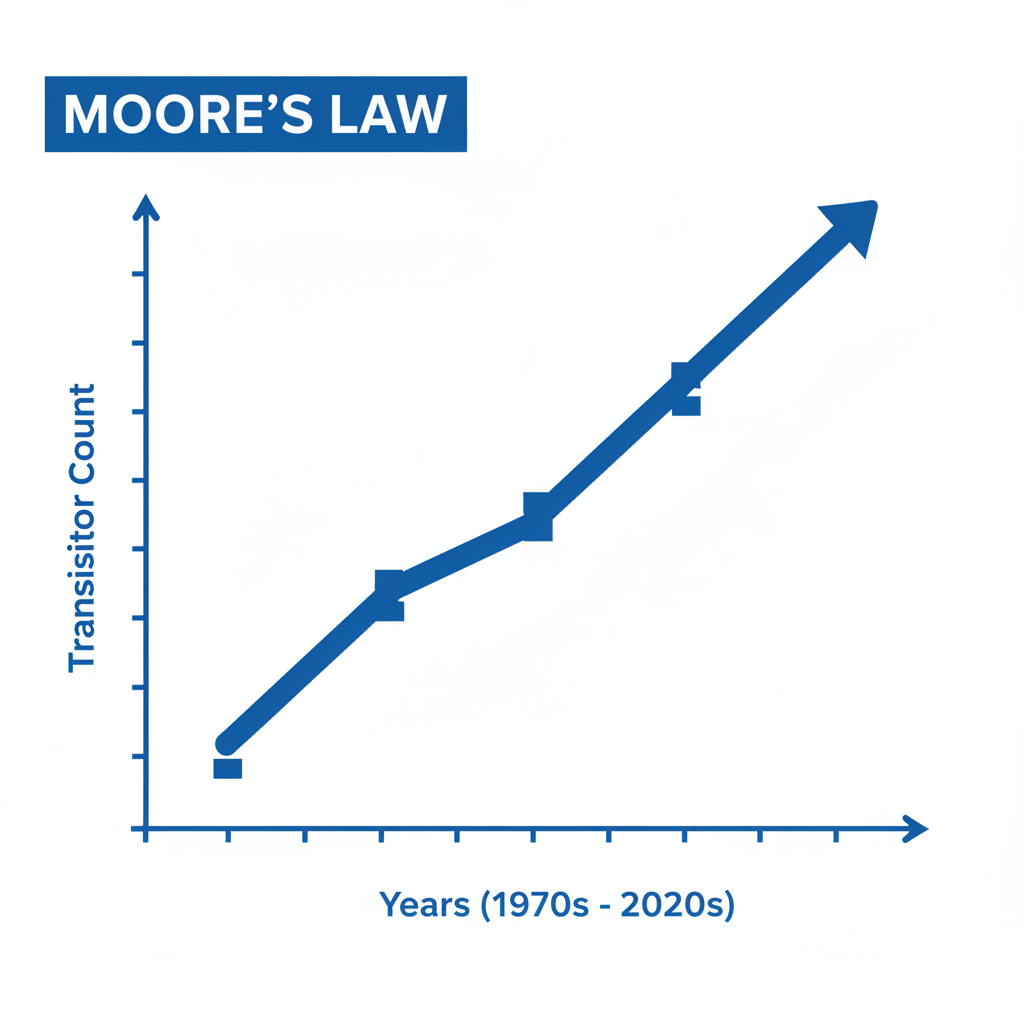
\includegraphics[width=\linewidth]{resources/8_great_ideas_of_computer_architecture/moores_law.png}
\end{minipage}

\bigskip

\subsection{Use Abstraction to Simplify Design}

\begin{minipage}[t]{0.7\linewidth}
Both computer architects and programmers had to invent techniques to make themselves more productive, for otherwise design time would lengthen as dramatically as resources grew by \textit{Moore's Law}. A major productivity technique for hardware and software is to use \textbf{abstractions} to represent the design at different levels of representation; lower-level details are hidden to offer a simpler model at higher levels. We'll use the abstract painting icon to represent this second great idea.
\end{minipage}
\hfill
\begin{minipage}[t]{0.28\linewidth}
    \centering
    
\includegraphics[width=\linewidth]{resources/8_great_ideas_of_computer_architecture/abstraction.png}
\end{minipage}

\bigskip

\subsection{Make the Common Case Fast}

\begin{minipage}[t]{0.7\linewidth}
Making the \textbf{common case fast} will tend to enhance performance better than optimizing the rare case. Ironically, the common case is often simpler than the rare case and hence is often easier to enhance. This common sense advice implies that you know what the common case is, which is only possible with careful experimentation and measurement. We use a sports car as the icon for making the common case fast, as the most common trip has one or two passengers, and it's surely easier to make a fast sports car than a fast minivan.
\end{minipage}
\hfill
\begin{minipage}[t]{0.28\linewidth}
    \centering
    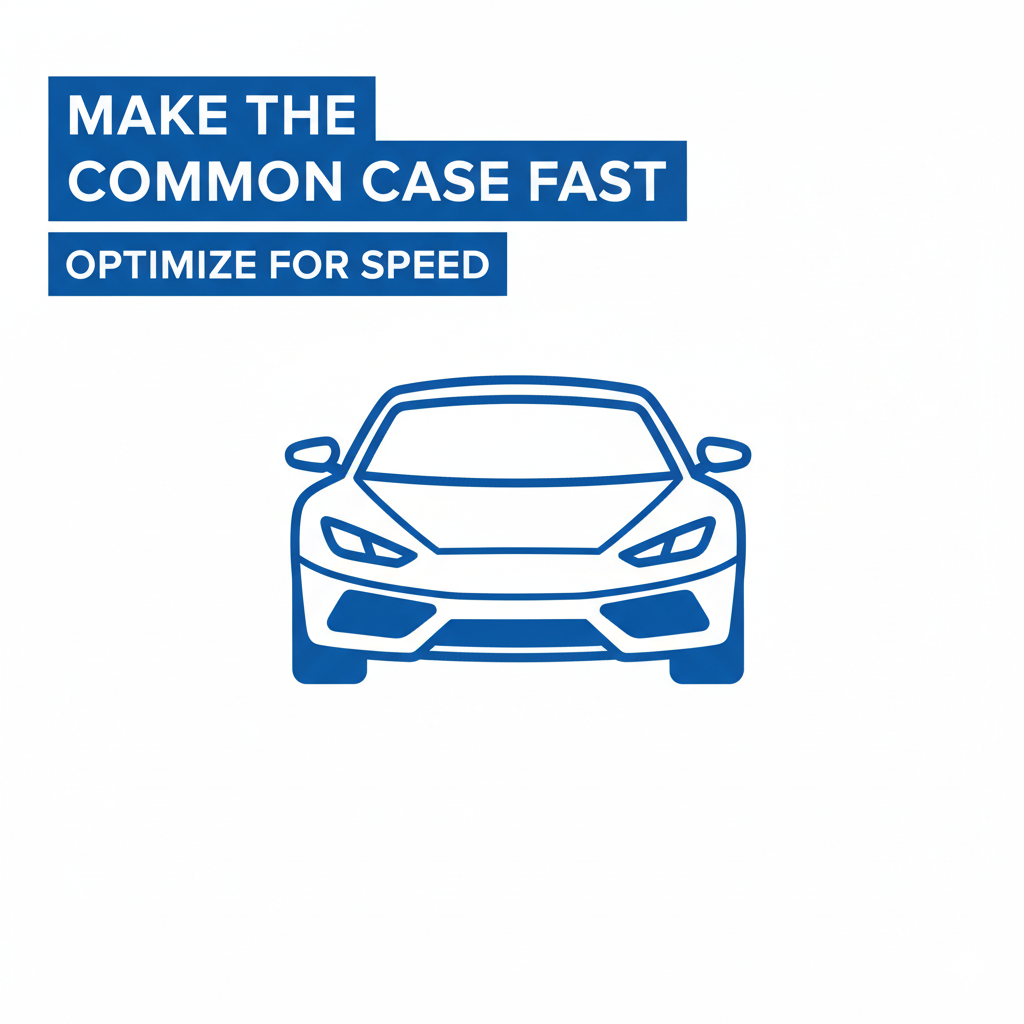
\includegraphics[width=\linewidth]{resources/8_great_ideas_of_computer_architecture/common_case_fast.png}
\end{minipage}

\bigskip

\subsection{Performance via Parallelism}

\begin{minipage}[t]{0.7\linewidth}
Since the dawn of computing, computer architects have offered designs that get more performance by performing operations in parallel. We use the multiple jet engines of a plane as our icon for \textbf{parallel performance}.
\end{minipage}
\hfill
\begin{minipage}[t]{0.28\linewidth}
    \centering
    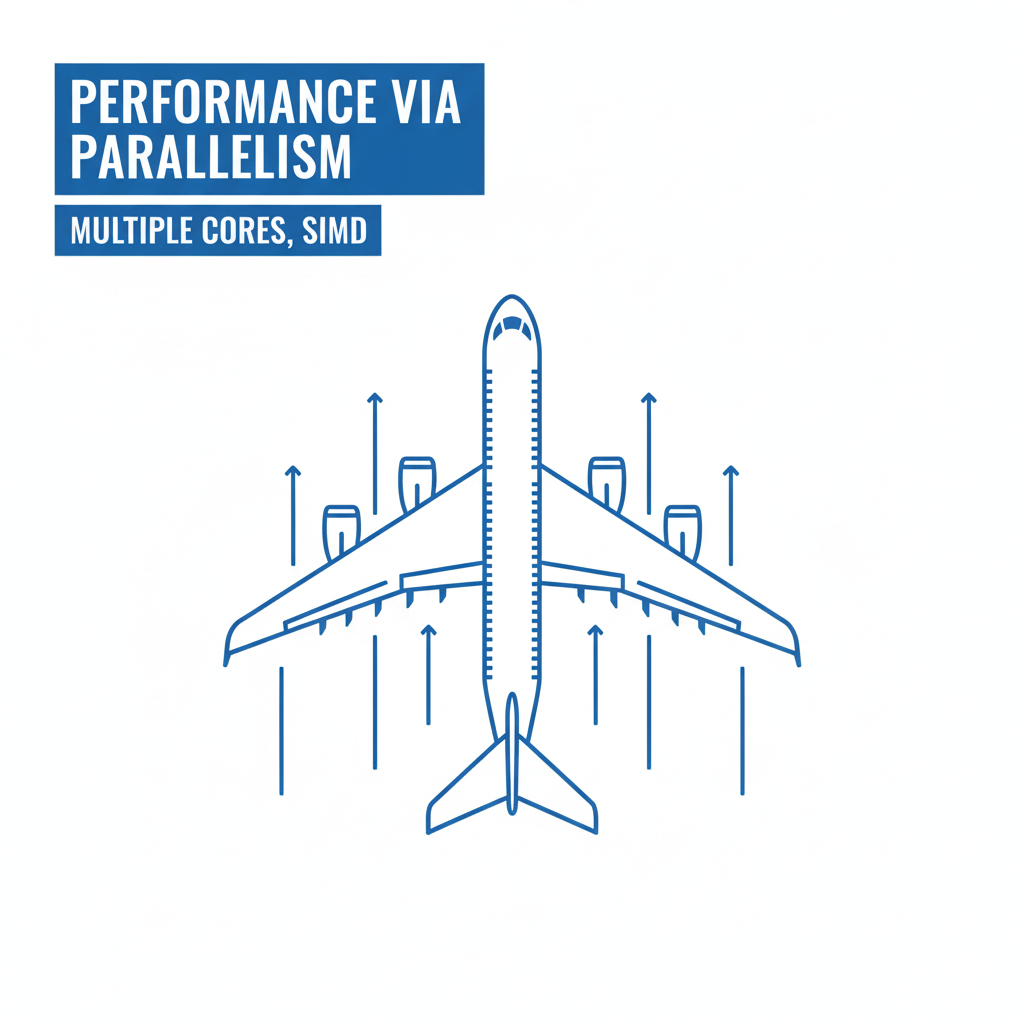
\includegraphics[width=\linewidth]{resources/8_great_ideas_of_computer_architecture/perf_via_parallelism.png}
\end{minipage}

\bigskip

\subsection{Performance via Pipelining}

\begin{minipage}[t]{0.7\linewidth}
A particular pattern of parallelism is so prevalent in computer architecture that it merits its own name: \textbf{pipelining}. For example, before fire engines, a "bucket brigade" would respond to a fire, which many cowboy movies show in response to a dastardly act by the villain. The townsfolk form a human chain to carry a water source to fire, as they could much more quickly move buckets up the chain instead of individuals running back and forth. Our pipeline icon is a "sequence" of pipes, with each section representing one stage of the pipeline.
\end{minipage}
\hfill
\begin{minipage}[t]{0.28\linewidth}
    \centering
    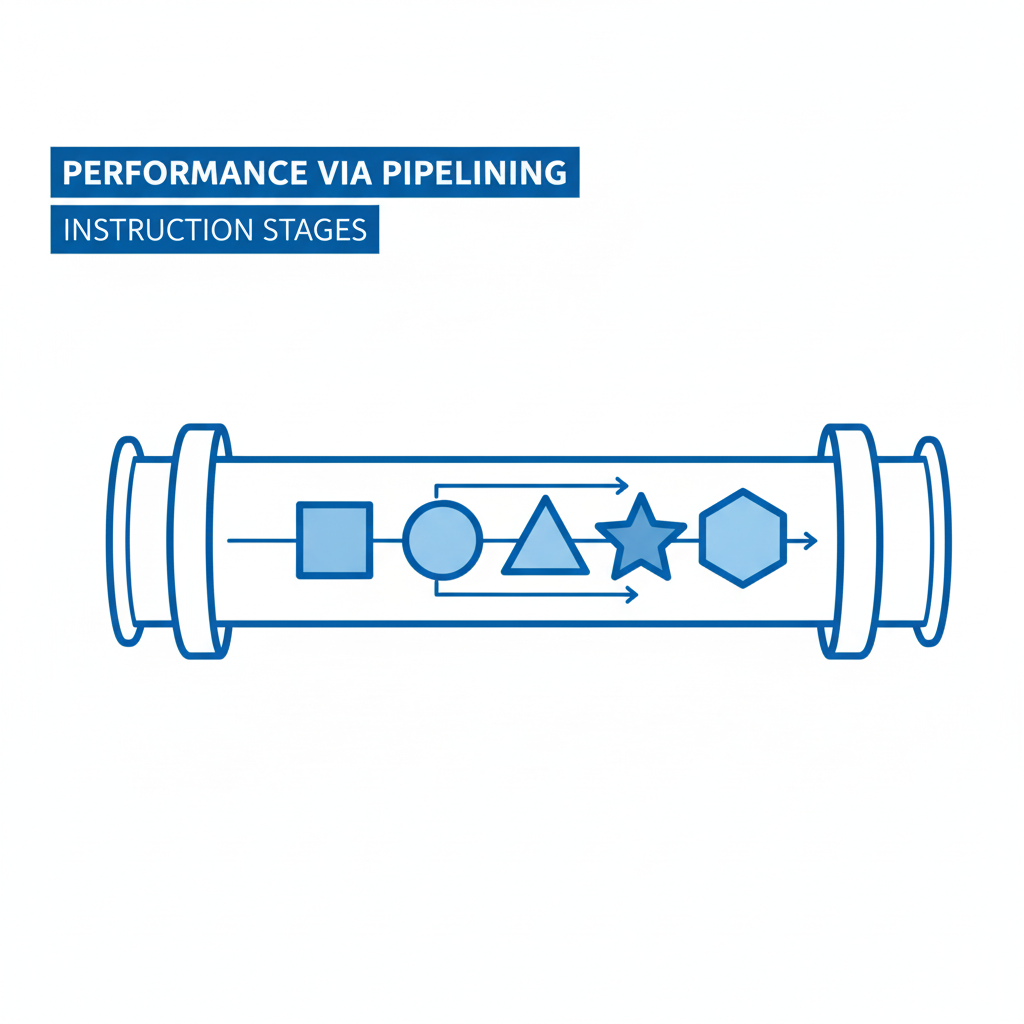
\includegraphics[width=\linewidth]{resources/8_great_ideas_of_computer_architecture/perf_via_pipelining.png}
\end{minipage}

\bigskip

\subsection{Performance via Prediction}

\begin{minipage}[t]{0.7\linewidth}
Following the saying that it can be better to ask for forgiveness than to ask for permission, the final great idea of performance is \textbf{prediction}. In some cases it can be faster on average to guess and start working rather than wait until you know for sure, assuming that the mechanism to recover from a misprediction is not too expensive and your prediction is relatively accurate. We use the fortune-teller's crystal ball as our prediction icon.
\end{minipage}
\hfill
\begin{minipage}[t]{0.28\linewidth}
    \centering
    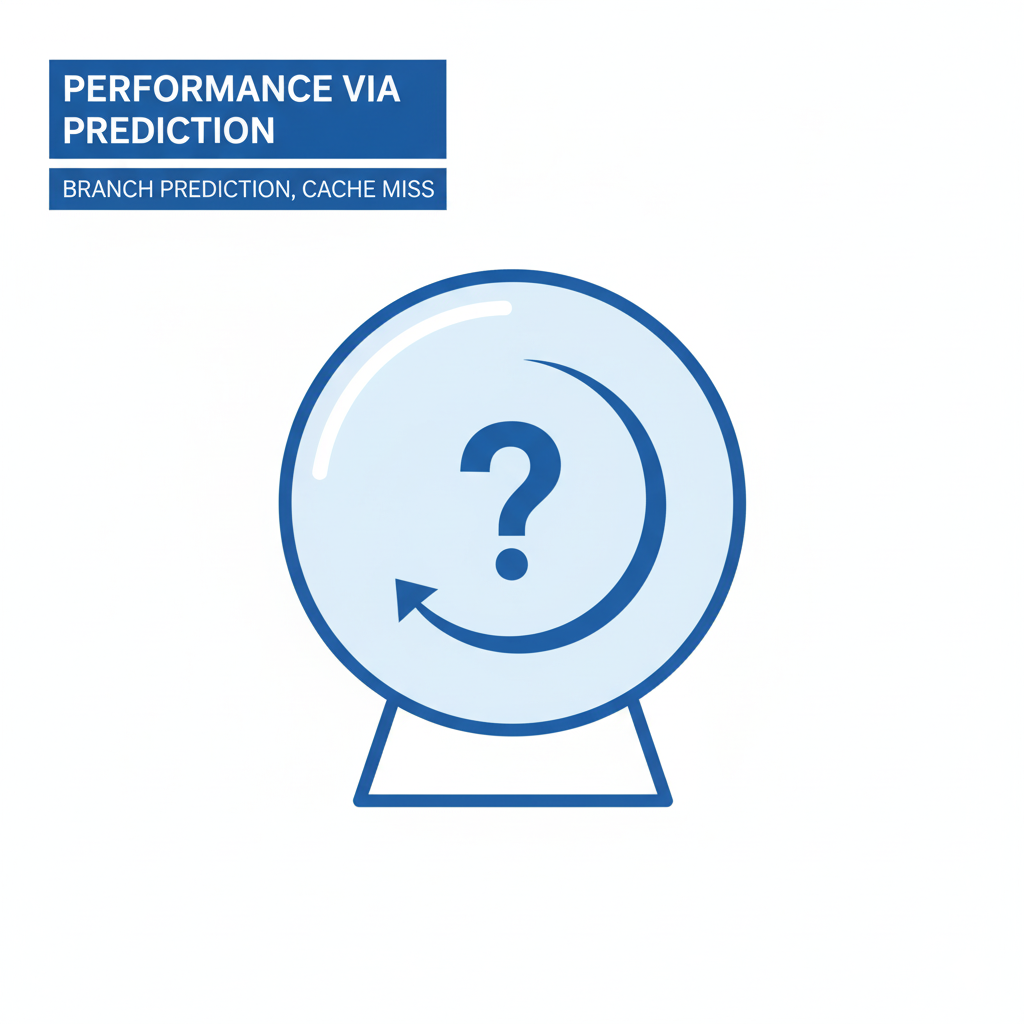
\includegraphics[width=\linewidth]{resources/8_great_ideas_of_computer_architecture/perf_via_prediction.png}
\end{minipage}

\bigskip

\subsection{Hierarchy of Memories}

\begin{minipage}[t]{0.7\linewidth}
Programmers want memory to be fast, large, and cheap, as memory speed often shapes performance, capacity limits the size of problems that can be solved, and the cost of memory today is often the majority of computer cost. Architects have found that they can address these conflicting demands with a \textbf{hierarchy of memories}, with the fastest, smallest, and most expensive memory per bit at the top of the hierarchy and the slowest, largest, and cheapest per bit at the bottom. Caches give the programmer the illusion that main memory is nearly as fast as the top of the hierarchy and nearly as big and cheap as the bottom of the hierarchy. We use a layered triangle icon to represent the memory hierarchy. The shape indicates speed, cost, and size: the closer to the top, the faster and more expensive per bit the memory; the wider the base of the layer, the bigger the memory.
\end{minipage}
\hfill
\begin{minipage}[t]{0.28\linewidth}
    \centering
    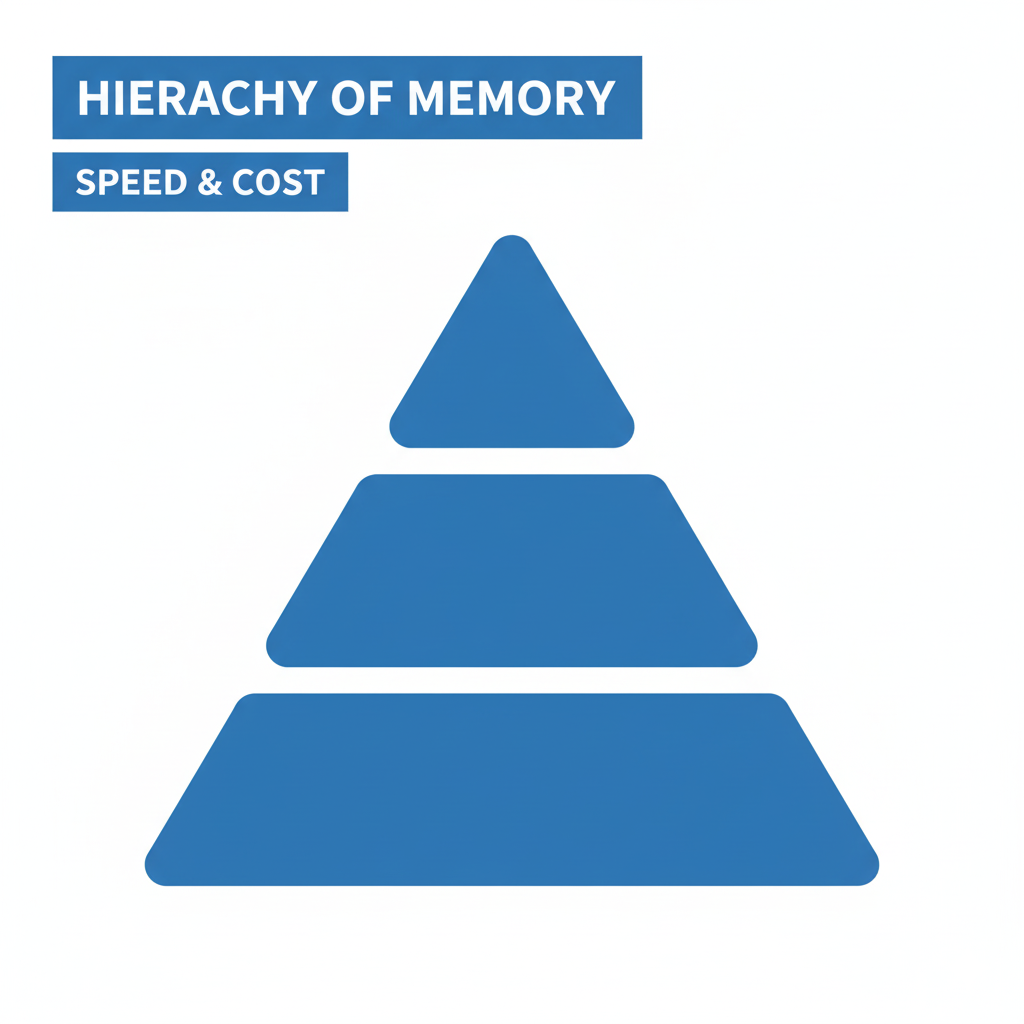
\includegraphics[width=\linewidth]{resources/8_great_ideas_of_computer_architecture/hierarchy_of_mem.png}
\end{minipage}

\bigskip

\subsection{Dependability via Redundancy}

\begin{minipage}[t]{0.7\linewidth}
Computers not only need to be fast; they need to be dependable. Since any physical device can fail, we make systems \textbf{dependable} by including redundant components that can take over when a failure occurs \textit{and} to help detect failures. We use the tractor-trailer as our icon, since the dual tires on each side of its rear axels allow the truck to continue driving even when one tire fails.
\end{minipage}
\hfill
\begin{minipage}[t]{0.28\linewidth}
    \centering
    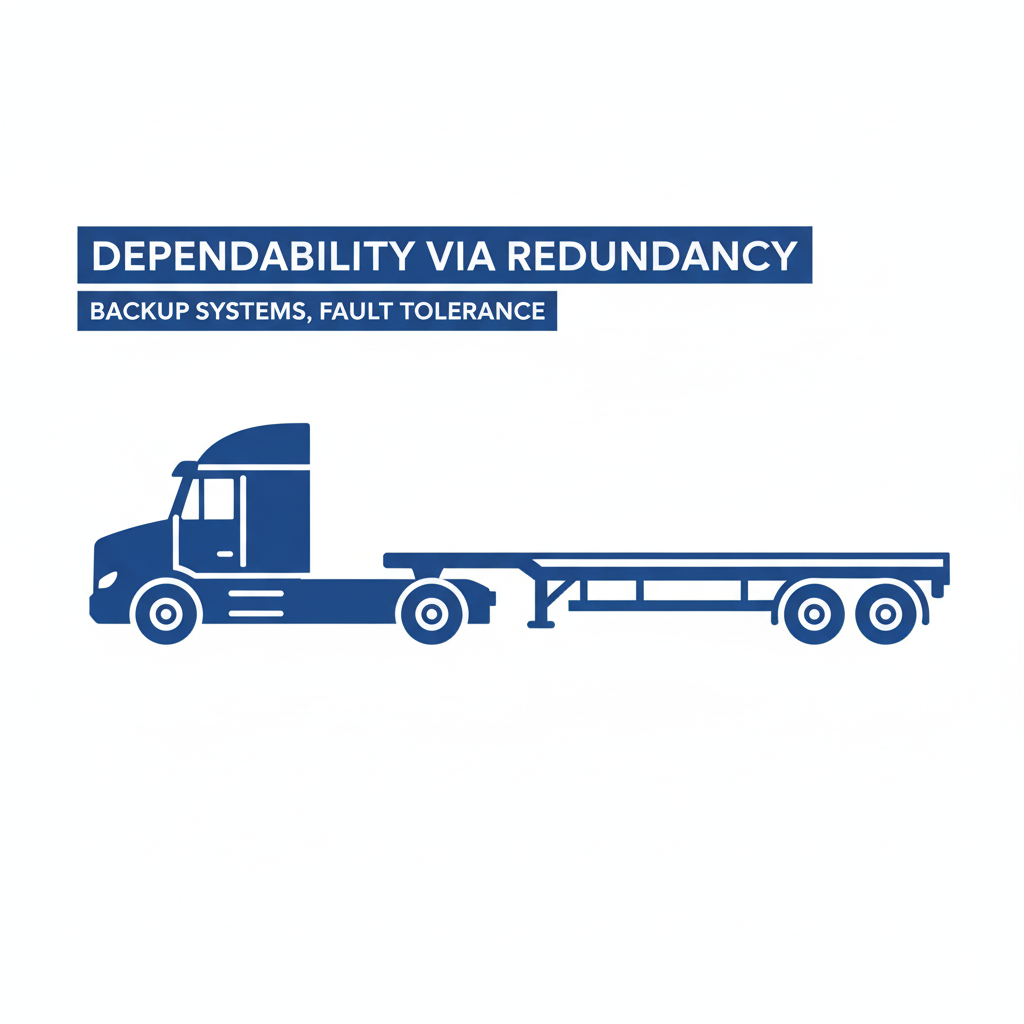
\includegraphics[width=\linewidth]{resources/8_great_ideas_of_computer_architecture/depend_via_redundancy.png}
\end{minipage}


\begin{lstlisting}[language=]
\end{lstlisting}

\begin{lstlisting}[language=]
\end{lstlisting}

\end{document}